%SourceDoc ../YourName-Dissertation.tex
\vspace*{-80mm}
\chapter{Solution Methods}
\label{chapter3:Solution Methods}

	\section{Residual Formulation}
	    
    A residual is simply the difference between the value at some future time
    $n+1$ and the value at the current iteration $k$ \cite{kelly1995}. This can
    be applied to desired variables as shown in equations
    \eqref{eq:residual_def:P}, \eqref{eq:residual_def:h},
    \eqref{eq:residual_def:u}, and \eqref{eq:residual_def:rho}. Residuals can
    also be applied to the conservation equations by substituting the definition
    of the residual variables into the conservation equations. This will
    effectively change any variables evaluated at $n+1$ to $k$. Each cell will
    have three residual variables and three residual equations. For the entire
    solution, we will then have a residual variable array $\delta X$, and a
    residual function array $F(X)$ which defines a linear system as seen in 
    equation \eqref{eq:linear_system}.
        
    \begin{equation}
    	\label{eq:residual_def:P}
    	\delta P_{i} = P^{n+1}_{i} - P^{k}_{i}
    \end{equation}
    
    \begin{equation}
    	\label{eq:residual_def:h}
    	\delta h_{i} = h^{n+1}_{i} - h^{k}_{i}
    \end{equation}
    
    \begin{equation}
    	\label{eq:residual_def:u}
    	\delta u_{i+\frac{1}{2}} = u^{n+1}_{i+\frac{1}{2}} - u^{k}_{i+\frac{1}{2}}
    \end{equation}
    
    \begin{equation}
    	\label{eq:residual_def:rho}
    	\delta \rho_{i} = \rho^{n+1}_{i} - \rho^{k}_{i}
    \end{equation}
    
    \begin{equation}
    	\label{eq:linear_system}
    	J \delta X = - F(X)
    \end{equation}
    
    \section{Jacobian Construction}
    
    The Jacobian matrix is defined in equation \eqref{eq:jac_def} as the derivative
    of each response of the function $F_{j}$ with respect to each variable $X_{i}$.
    The derivative can be calculated numerically as shown by equation
    \eqref{eq:jac_numerical} where $\epsilon$ is a small numerical value. For
    COBRA-TF the equations are linear, and this numerical approximation
    of the Jacobian matrix is exact. This should produce the same jacobian
    matrix that COBRA-TF currently generates analytically. 
    
    \begin{equation}
    	\label{eq:jac_def}
    	J_{i,j}=\frac{ \partial F_{j}(X)}{\partial X_{i}}
    \end{equation}
    
    \begin{equation}
    	\label{eq:jac_numerical}
    	J_{i,j}  \approx \frac{F_{j}(X_{i}+\epsilon)-F_{j}(X)}{\epsilon}
    \end{equation}
    
    To build the jacobian matrix, an object oriented class was created that
    contains three arrays. An array that points to the residual functions, an
    array that points to the position within a target variable array, and an
    array that has the index that the function is to be evaluated at. These
    lists can be appended to in any order, but have to be appended all at the
    same time so that variables and functions must correspond with each other.
    Then to construct the jacobian matrix, the residual function and residual
    variable arrays can each be looped over to numerically build the jacobian
    matrix as seen in figure \ref{fig:Jacobian_Setup}. 
    
    \begin{figure}[!h]
    	\centering
    	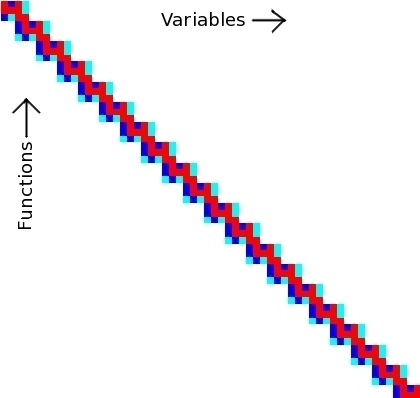
\includegraphics[width=0.30\textwidth]{images/Jacobian_Setup}
    	\caption{Structure of the jacobian matrix for single phase liquid}
    	\label{fig:Jacobian_Setup}
    \end{figure}


	The explicitly coupled solid liquid Jacobian matrix can be seen in figure
	\ref{fig:Explicit-Diagram}, where blue values represent negative entries and
	red values positive entries. The black lines were drawn on top of the image to
	represent artificial boundaries between the liquid Jacobian matrix in the top
	left corner and the solid Jacobian matrix in the top right corner. The fluid
	Jacobian matrix contains 3 conservation equations for every axial level. The
	liquid function residuals are appended in the order of mass conservation,
	energy conservation, and momentum conservation for each axial level. These
	correspond the pressure, enthalpy, and velocity at each axial level. The liquid
	Jacobian matrix can be evaluated as either semi-implicit or fully implicit. The
	solid Jacobian matrix contains 1 energy conservation equation for each node in
	the rod. Since axial and azimuthal conduction are not computed, each radial
	level is computed separately from the rest. This can be seen by the lack of
	cross terms in the Jacobian matrix at each axial level. The Jacobian matrix on
	the right is an implicit coupling between the implicit liquid Jacobian matrix
	and the implicit solid matrix. The cross terms in the top right corner
	represent the effect of the wall temperature on the energy equation in the
	liquid Jacobian matrix. The terms on the bottom left represent the effects of
	pressure, enthalpy, and velocity on the energy equation in the solid Jacobian
	matrix. The implicit matrix is unconditionally stable, allowing for time steps
	greater than the material Courant limits. Once the coupled Jacobian matrix is
	constructed, it is solved using the linear Krylov solver \cite{kelly2003} from
	PETSc \cite{PETSc}. The residuals for each of the conservation equations are
	then L2 normalized over the domain to determine the convergence of the system.
	
	\begin{figure}[!h]
    	\centering
    	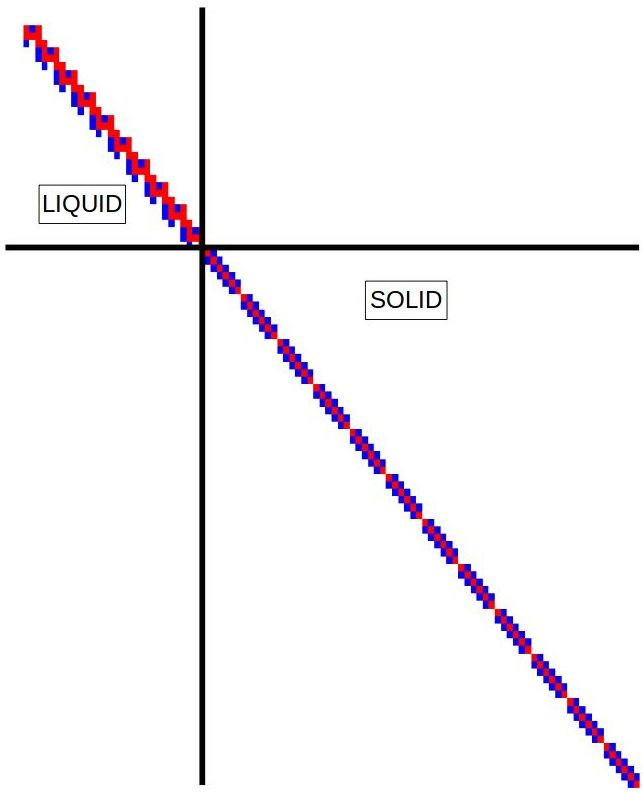
\includegraphics[width=0.30\textwidth]{images/Explicit-Diagram.jpg}
    	\caption{Structure of jacobian matrix for single phase liquid
    	explicitly coupled to solid conduction}
    	\label{fig:Explicit-Diagram}
    \end{figure}
    
    \begin{figure}[!h]
    	\centering
    	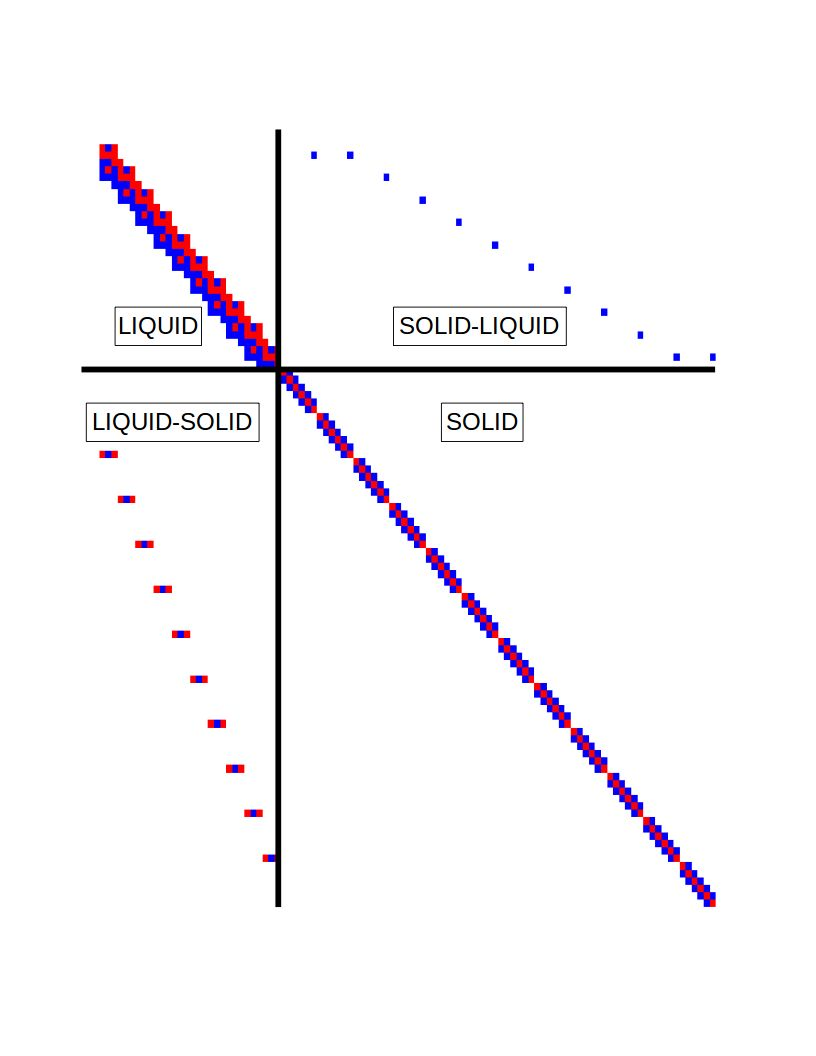
\includegraphics[width=0.30\textwidth]{images/Implicit-Diagram.jpg}
    	\caption{Structure of the jacobian matrix for single phase liquid
    	implicitly coupled to solid conduction}
    	\label{fig:Implicit-Diagram}
    \end{figure}
    
    Numerically building the matrix in this fashion can be very computationally
    expensive. An easy way to optimize the construction of the matrix, is to not
    compute the indexes which are known to be zero. An optional optimization
    flag was added to the code that allows for the non-zero structure to be
    remebered after the first construction, and following constructions only
    compute entries that were previously non-zero. This drastically decreases
    computations cost, but at the risk of serious potential error in the event
    of previously zero entries becoming non-zero later in the problem. For the
    verification problems covered in this work, this does not occur and
    therefore this optimization method is appropriate. Other optimization work
    could be in the parallelization of the construction and solution of the
    Jacobian matrix similar to what was done for the original version of CTF
    \cite{Salko2014}.
   
    
    
    
    






